\chapter{Kajian Pustaka}
Tugas akhir ini membahas perancangan sistem pengawasan jantung. Untuk mendirikan landasan berfikir, bab ini akan membahas fakta dan teori yang berkaitan dengan perancangan sistem tersebut.

\section{Sistem yang Ada dan Riset Terkait}
\textit{Monitoring} jantung bukanlah hal yang baru. Hal ini ditandai dengan banyaknya produk dan riset mengenai \textit{monitoring} jantung.

\subsection{Produk Monitoring Jantung di Pasaran}
Meningkatnya kesadaran masyarakat akan CVDs mendorong banyak perusahaan untuk membuat produk \textit{monitoring} jantung \textit{portable}. Perusahaan seakan berlomba memproduksi alat monitoring baik yang berstandar medis untuk penggunaan rawat intesif maupun yang tidak berstandar medis untuk penggunaan sehari hari. Selain produk berbentuk alat (\textit{hardware}), produk berbentuk program (\textit{software}) yang hanya memanfaatkan \textit{LED flash} di kamera \textit{smartphone} sebagai sensor PPG juga banyak ditemukan[xx-xx-xx].

Salah satu perusahaan yang ikut memproduksi alat \textit{monitoring} ialah perusahaan yang terkenal dengan jam tangan pintarnya yaitu Fitbit. Fitbit mengeluarkan "Fitbit Blaze" pada tahun 2016[xx]. Fitbit Blaze dilengkapi dengan PPG pada bagian belakangnya. Fitbit Blaze juga dilengkapi aplikasi Android untuk melihat hasil \textit{monitoring} secara lengkap. Fitbit Blaze terhubung kepada ponsel Android menggunakan Bluetooth. Fitbit Blaze dirancang sebagai pelengkap \textit{lifestyle} agar penggunanya dapat menggunakannya sehari hari. Hasil \textit{monitoring} dari Fitbit dapat dibagikan kepada siapapun setelah sebuah \textit{record} selesai direkam.

Sama seperti Fitbit, perusahaan raksasa dari Korea, Samsung, juga mengeluarkan produk \textit{lifestyle} berupa sebuah jam tangan pintar yang dapat melakukan \textit{monitoring} jantung. Produk milik Samsung diberi nama "Gear S3" (gambar \ref{fig:device_example} a) dan diluncurkan pada tahun 2017 [xx]. Gear S3 dilengkapi sensor PPG di bagian belakangnya. Gear S3 dapat terhubung ke jaringan secara \textit{wireless} dengan menggunakan koneksi \textit{Bluetooth} dan \textit{Wi-Fi}. Hasil \textit{monitoring} dari Gear S3 hanya dapat dilihat pada layar yang melengkapinya.

PT. Endo Indonesia, sebuah perusahaan peralatan medis asal Indonesia, juga membuat alat \textit{monitoring} jantung. Tidak seperti Fitbit dan Samsung, produk besutan Endo ditujukan untuk pemakaian medis. Endo memproduksi Holter monitor "EDAN SE-2003" (gambar \ref{fig:device_example} b) dan Pulse Oximeter "EDAN H-10" (gambar \ref{fig:device_example} c). "SE-2003" menggunakan sensor berjenis ECG dan mampu melakukan \textit{monitoring} pada 3 \textit{channel} sekaligus [xx]. Berbeda dengan "SE-2003", "H-10" menggunakan PPG . Pulse Oximeter "H-10", sesuai namanya, selain mampu \textit{monitoring} jantung (\textit{Pulse}) juga mampu mengukur kadar oxigen dalam darah (\textit{Oximeter}). "H-10" merupakan pulse oximeter yang diletakkan pada ujung jari (\textit{fingertip}). Hasil \textit{monitoring} holter monitor dan pulse oximeter Endo dapat dilihat pada layar produk tersebut dan aplikasi desktop yang menyertainya.

Produk berupa aplikasi/\textit{software} (gambar \ref{fig:device_example} d) dapat ditemukan dengan mudah pada toko aplikasi \textit{virtual} (\textit{playstore}, \textit{app store}, dll). Penulis melakukan studi perbandingan terhadap 10 aplikasi teratas (Juli 2017) dengan kata kunci pencarian "Heart Rate" pada \textit{Play Store} (toko aplikasi virtual ponsel Android). Setelah membandingkan aplikasi tersebut, tidak ditemukan aplikasi yang memiliki fitur \textit{monitoring} lengkap untuk menyelesaikan permasalahan yang diajukan pada bab sebelumnya. Hasil perbandingan terhadap 10 aplikasi ini dicantumkan pada tabel \ref{table:app_comparison}

Semua produk yang disebutkan sebelumnya tidaklah \textit{Open Source}. Sehingga tidak dimungkinkan untuk merubah spesifikasi kinerja produk seperti menaikkan \textit{sample rate} atau mengganti algorima penghitung detak jantung. Walaupun tidak \textit{Open Source}, baik Fitbit dan Samsung memberikan \textit{Application Programming Interface} (\textit{API}) untuk memudahkan pengembang perangkat lunak membuat sistem yang menggunakan produk mereka [xx][xx]. API tersebut memungkinkan pengembang mengambil semua data sensor yang tertanam pada produk. Untuk kasus \textit{monitoring} jantung, pengembang dapat mengambil bentuk gelombang jantung dan BPM dari produk. Sedangkan, Endo tidak menyediakan API sama sekali. Sehingga, untuk mengakses pengukuran dari produk Endo akan sangat sulit untuk dilakukan (mungkin dilakukan dengan \textit{Reverse Engineering}). Rangkuman perbedaan produk berupa alat dapat dilihat pada tabel \ref{table:product_comparison}

\begin{figure}[H]
    \centering
	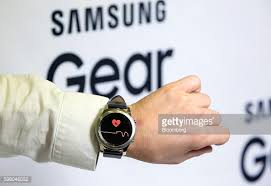
\includegraphics[scale=0.4]{images/gears3.jpg}
	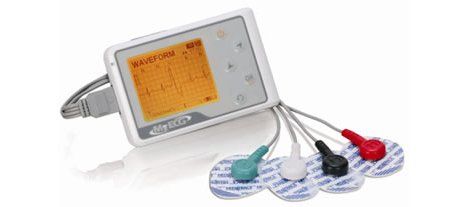
\includegraphics[scale=0.3]{images/ecg_1.jpg}	
	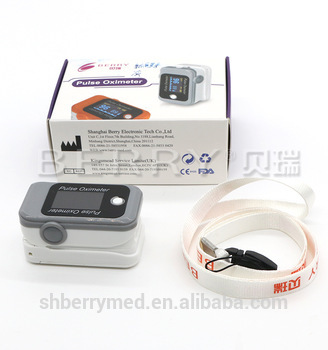
\includegraphics[scale=1]{images/ppg_clip.jpg}
	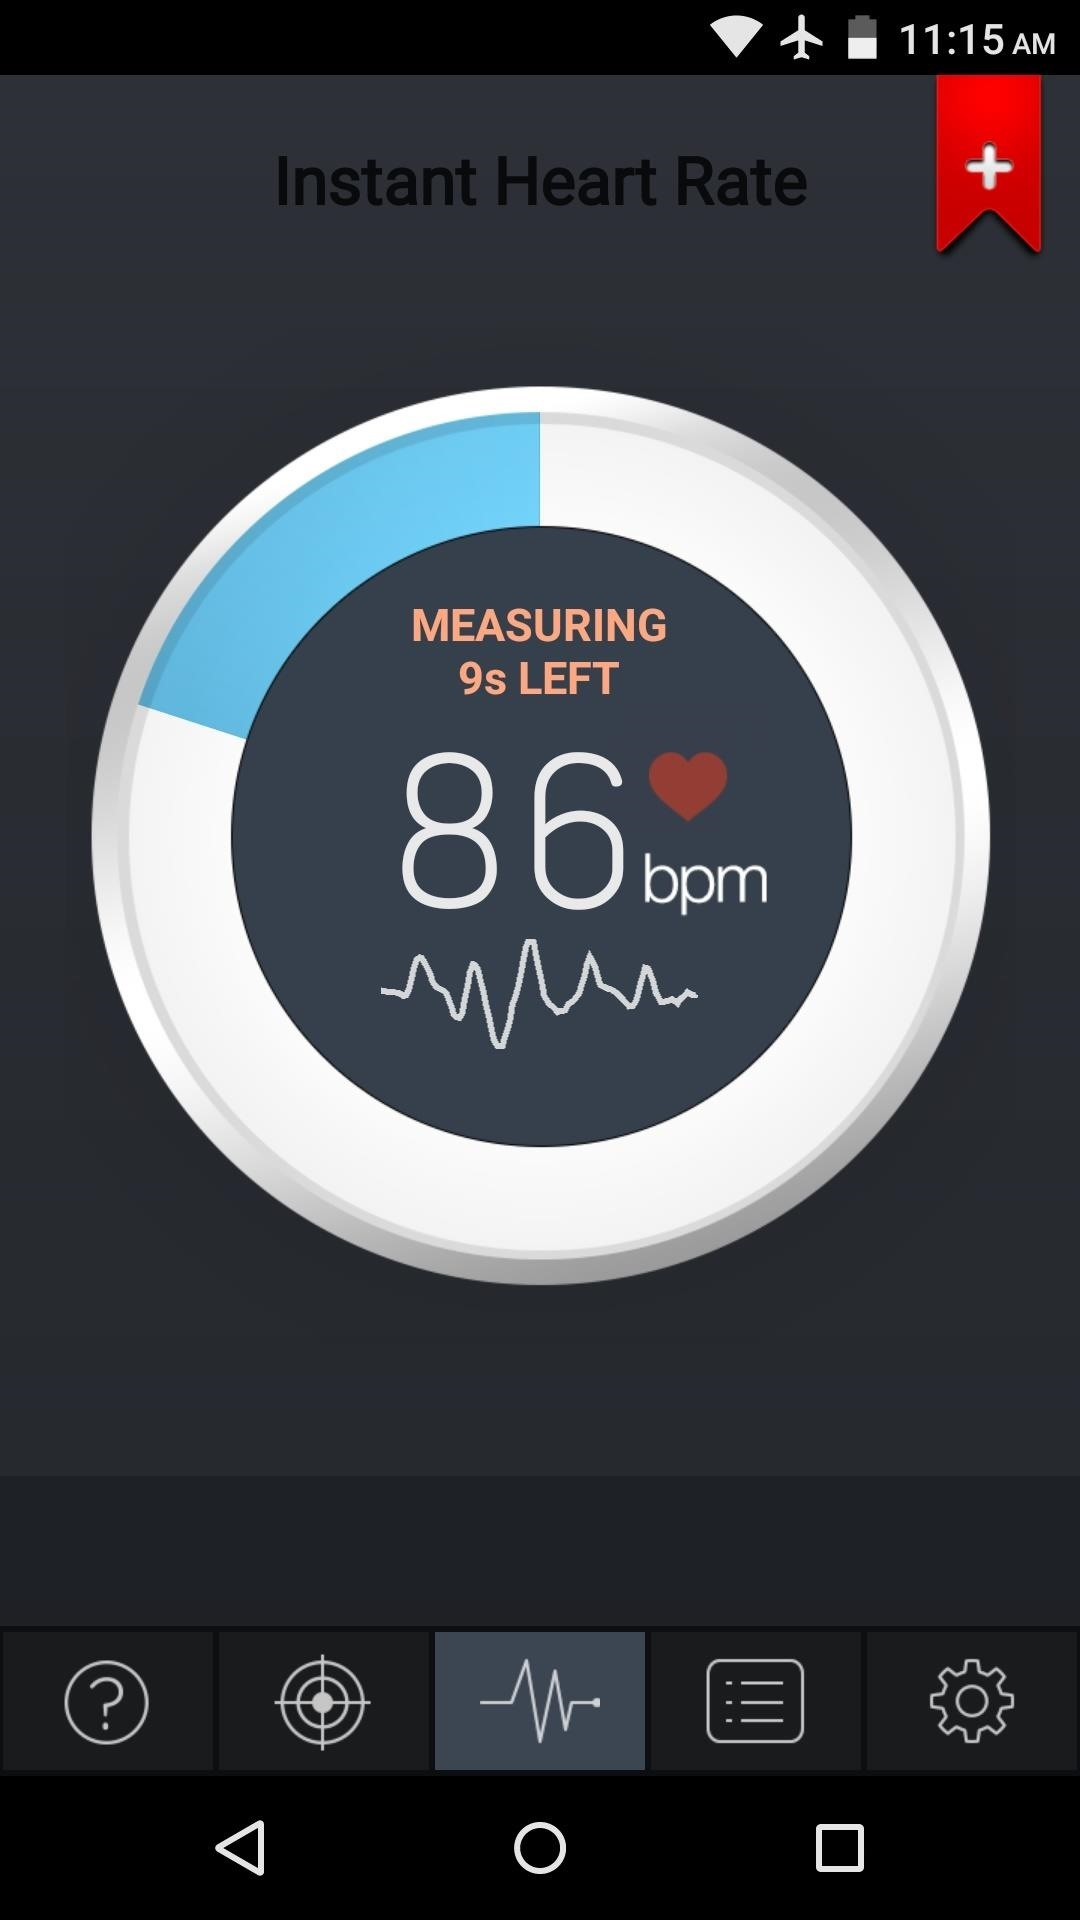
\includegraphics[scale=0.05]{images/heart_app1.jpg}
    \caption{a) Samsung Gear S3; b) Holter Monitor; c) Fingertip Pulse Oximeter; d) Heart Rate App}
    \label{fig:device_example}
\end{figure}

\begin{table}[H]
	\centering
	\begin{tabular}{|l|L{4cm}|c|L{0.5cm}|L{0.5cm}|L{0.5cm}|L{0.5cm}|L{0.5cm}|L{0.5cm}|L{0.5cm}|L{0.5cm}|}
		\hline
		\rowcolor{gray}
		\textbf{No} & \textbf{Aplikasi} & \textbf{Sen} & \multicolumn{8}{c}{\textbf{Fitur}} \\
		\rowcolor{gray}
		 & & \textbf{sor} & A & B & C & D & E & F & G & H \\
		\hline
		1 & Instant Heart Rate : Heart Rate \& Pulse Monitor & PPG & Y & N & Y & Y & N & Y & N & Y \\
		2 & iCare Health Monitor (BP \& HR) & PPG & Y & N & Y & N & N & Y & N & Y \\
		3 & Heart Rate Monitor(REPS) & PPG & Y & N & Y & Y & N & Y & N & Y \\
		4 & Runtastic Heart Rate Monitor \& Pulse Checker & PPG & Y & N & Y & N & N & Y & N & N \\
		5 & Cardiograph - Heart Rate Meter & PPG & Y & N & Y & Y & N & Y & N & Y \\
		6 & ASUS Heart Rate & PPG & N & N & N & N & N & Y & N & N \\
		7 & Samsung Health & PPG & Y & Y & N & N & N & Y & N & Y \\
		8 & Heart Rate Monitor(Meet Your Need Production) & PPG & N & N & N & N & N & Y & N & N \\
		9 & \textbf{MobECG} & \textbf{ECG} & N & Y & Y & Y & N & Y & N & N \\		
		10 & \textbf{CMS50Dplus} & \textbf{ECG} & N & Y & Y & Y & N & Y & N & N \\
		\hline
	\end{tabular}
	\caption{Perbandingan 10 Aplikasi Monitoring Jantung di Play Store}
	\label{table:app_comparison}
\end{table}

Ket: \\
A = Identitas User \\
B = Real Time Monitoring \\
C = Melihat Gelombang Jantung \\
D = Merekam Gelombang Jantung \\
E = Multiuser Monitoring \\
F = Deteksi BPM \\
G = Aritmia Alert \\
H = Share Result via Network \\

\begin{table}[H]
	\centering
	\begin{tabular}{|l|L{3cm}|c|c|c|L{0.5cm}|L{0.5cm}|L{0.5cm}|L{0.5cm}|L{0.5cm}|L{0.5cm}|L{0.5cm}|L{0.5cm}|}
		\hline
		\rowcolor{gray}
		\textbf{No} & \textbf{Produk} & \textbf{Sen} & \textbf{Me} & \textbf{Op} & \multicolumn{8}{c}{\textbf{Fitur}} \\
		\rowcolor{gray}
		 & & \textbf{sor} & \textbf{dis} & \textbf{en} & A & B & C & D & E & F & G & H \\
		\hline
		1 & Fitbit Blaze & PPG & N & N & Y & Y & Y & Y & N & Y & N & Y \\
		2 & Samsung Gear S3 & PPG & N & N & Y & Y & Y & N & N & Y & N & Y \\
		3 & ENDO SE-2003 & ECG & Y & N & Y & Y & Y & Y & N & Y & N & N \\
		4 & ENDO H-10 & PPG & Y & N & Y & Y & Y & Y & N & Y & N & N \\
		\hline
	\end{tabular}
	\caption{Perbandingan Produk Berupa Alat}
	\label{table:product_comparison}
\end{table}

Ket: \\
A = Identitas User \\
B = Real Time Monitoring \\
C = Melihat Gelombang Jantung \\
D = Merekam Gelombang Jantung \\
E = Multiuser Monitoring \\
F = Deteksi BPM \\
G = Aritmia Alert \\
H = Share Result via Network \\

\subsection{Riset Terkait}
Analisis terhadap rekam jantung Untuk mengklasifikasian aritmia seorang dokter perlu melihat hasil rekam jantung seorang pasien seperti gambar \ref{fig:contoh_aritmia}, baik hasil rekam ECG maupun PPG. Akan sangat melelahkan jika seorang dokter secara terus menerus memeriksa rekam jantung seorang pasien. Oleh karena itu dibutuhkan sebuah algoritma yang dapat melakukan klasifikasi secara otomatis. 

Telah banyak penelitian yang dilakukan yang melakukan otomasi klasifikasi aritmia[xx]. Kini penelitian tersebut telah memiliki keakuratan yang cukup baik, mencapai 90\%, dengan berbagai macam metode dan ekstraksi fitur.

Pada tahun xxx, asme asme asem

Pada tahun xxx, asme asme asem

Pada tahun xxx, asme asme asem

Pada tahun xxx, asme asme asem

Pada tahun xxx, asme asme asem

Pada tahun xxx, asme asme asem

\begin{table}[H]
\centering
	\begin{tabular}{|c|c|c|c|c|}
	\hline
	\rowcolor{gray}
	\textbf{Judul} & \textbf{Penulis} & \textbf{Fitur} & \textbf{Metode}  & \textbf{Hasil}\\
	\cline{1-5}
	Penemuan bla bla adu adu & Alif Akbar & Titik R & Decisin & 90\% \\
	\cline{1-5}
	Penemuan bla bla adu adu & Alif Akbar & Titik R & Decisin & 90\% \\
	\cline{1-5}
	Penemuan bla bla adu adu & Alif Akbar & Titik R & Decisin & 90\% \\
	\hline
	\end{tabular}
	\caption{Perbandingan riset mengenai klasifikasi aritmia otomasis}
	\label{table:research_comparison}
\end{table}

\section{ECG dan PPG}
Terdapat 2 jenis sensor yang umum digunakan untuk melakukan \textit{monitoring} jantung, yaitu \textit{Electrocardiogram} (ECG) dan \textit{Photoplethysmogram} (PPG) seperti yang terlihat pada gambar \ref{fig:ecg_n_ppg}. Kedua jenis sensor ini menjadi pilihan utama dalam \textit{monitoring} jantung karena keduanya mengusung konsep \textit{non-invasive}. Sensor non-invasive memungkinkan melakukan pengambilan data tubuh tanpa perlu melukai/menusuk bagian tubuh tertentu. Secara umum ECG akan menghasilkan pengukuran lebih akurat dari pada PPG. Namun PPG lebih nyaman digunakan dalam jangka panjang dari pada ECG.

\begin{figure}[H]
    \centering
    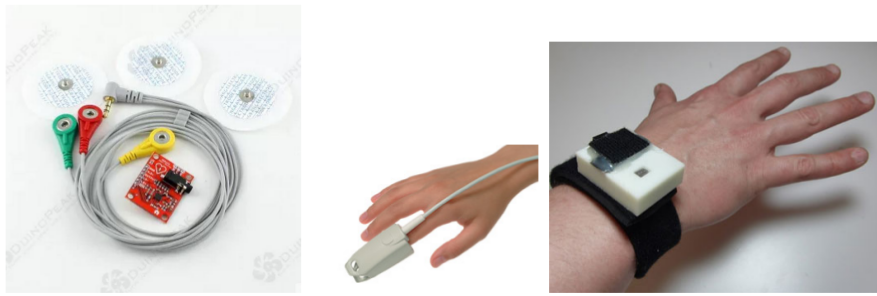
\includegraphics[scale=0.3]{images/sensors.png}
    \caption{a. Sensor ECG dengan 3 \textit{leads}; b. Sensor PPG ujung jari; c. Sensor PPG di pergelangan tangan}
    \label{fig:ecg_n_ppg}
\end{figure}

\subsection{Lokasi Penempatan Sensor}
\subsubsection{ECG}
ECG perlu melakukan pengukuran minimal di 3 lokasi. Hal ini disebabkan karena ECG secara langsung mengukur perubahan nilai kelistrikan yang dihasilkan tubuh. Untuk mengukur kelistrikan tubuh ECG memerlukan minimal 3 elektroda yaitu + (positif), - (negatif) dan N (netral), terlihat pada gambar \ref{fig:electrode3}. Untuk pengukuran lebih dari 3 titik, elektroda ECG dapat diletakkan pada posisi yang ditunjukkan gambar \ref{fig:multi_elctrode}.

\begin{figure}[H]
    \centering
    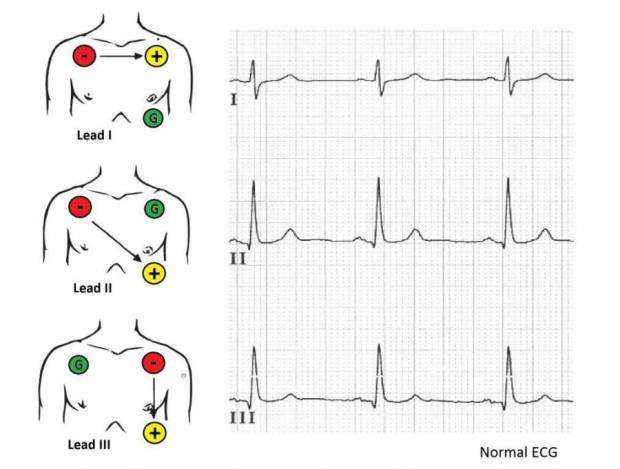
\includegraphics[scale=0.3]{images/3_ecg_place.jpg}
	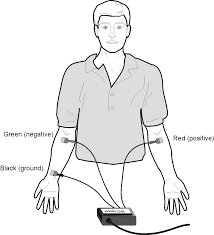
\includegraphics[scale=0.6]{images/3_ecg_place_2.png}    
    \caption{a. Penempatan 3 Elektroda di Dada, b. Penempatan 3 Elektroda di Tangan}
    \label{fig:electrode3}
	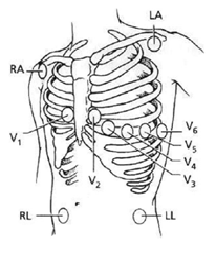
\includegraphics[scale=0.8]{images/multi_ecg.png}
    \caption{Lokasi Penempatan Lebih 3 titik}
    \label{fig:multi_elctrode}
\end{figure}

\subsubsection{PPG}
PPG dapat melakukan pengukuran hanya di satu lokasi. Hal ini disebabkan karena PPG mengukur tingkat penyerapan cahaya oleh darah, sedangkan pembuluh darah menjalar ke seluruh tubuh. Namun, untuk menghasilkan pengukuran maksimal PPG perlu diletakkan di lokasi tubuh yang pembuluh darah dekat dengan permukaan kulit \cite{ppg_placement}\cite{ppg_placement2}. Beberapa lokasi tubuh yang sesuai kriteria tersebut terdapat pada ujung jari, pergelangan tangan, lengan atas, leher, dan daun kuping.


\subsection{Titik Fiducial}
Untuk mengenali sebuah detak jatung pada rekam ECG maupun PPG diperlukan untuk mencari titik titik \textit{fiducial} (pembanding). Kemunculan titik fiducial menandakan adanya siklus \textit{beat} (detak) pada waktu kemunculan titik tersebut. Sebuah siklus sinyal ECG dapat dilihat dari beberapa titik fiducial yaitu P-QRS-T, seperti terlihat pada gambar \ref{fig:ecg_points}. Sedangkan siklus sinyal PPG dilihat dari siklus Diastolic-Systolic-Dicrotic seperti terlihat pada gambar \ref{fig:ppg_points}

\begin{figure}[H]
    \centering
    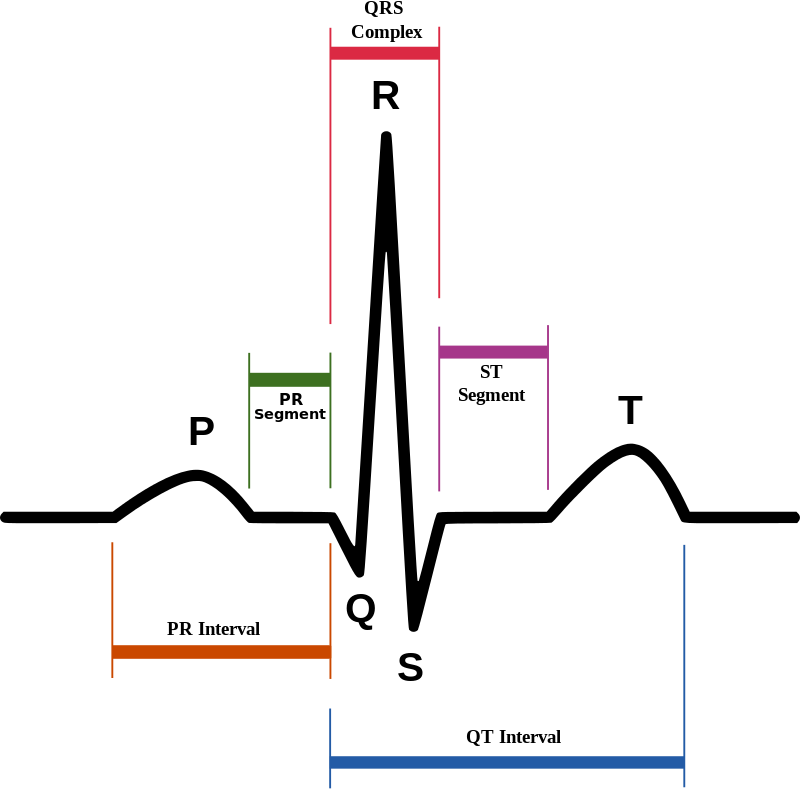
\includegraphics[scale=0.2]{images/ecg_points.png}
    \caption{Sinyal ECG berdasarkan titik fiducial}
    \label{fig:ecg_points}
	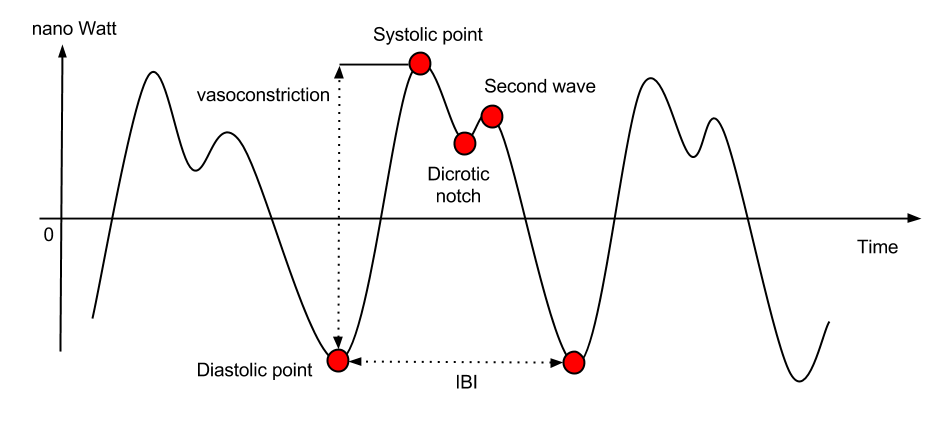
\includegraphics[scale=0.3]{images/PPG2.png}
    \caption{Sinyal PPG berdasarkan titik fiducial}
    \label{fig:ppg_points}
\end{figure}


\subsection{Bentuk Sinyal}
Dapat dilihat, pada gambar \ref{fig:ecg_vs_ppg}, dengan mudah bahwa sinyal bentukan dari PPG dengan ECG berbeda secara morfologi (bentuk)\cite{ppg_vs_ecg}. Namun, karena sumber sinyal yang sama (dari jantung) siklus PPG dan ECG dapat disinkronisasi (saling dipetakan) berdasarkan titik R pada ECG dan puncak sistolik pada PPG seperti gambar \ref{fig:ecg_vs_ppg2} \cite{ecg_syncro}. Perbedaan waktu kemunculan R dan Sistolik dikenal sebagai \textit{Pulse Arrival Time} (PAT). PAT dapat digunakan sebagai parameter mengukur tekanan darah, yang mana tidak dicakup pada tugas akhir ini.

\begin{figure}[H]
    \centering
    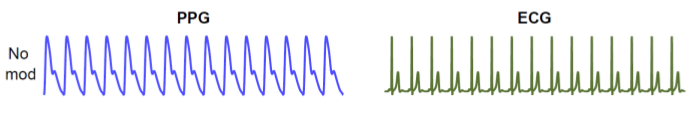
\includegraphics[scale=0.6]{images/ecg_vs_ppg.png}
    \caption{Perbandingan sinyal ideal PPG dan ECG}
    \label{fig:ecg_vs_ppg}
	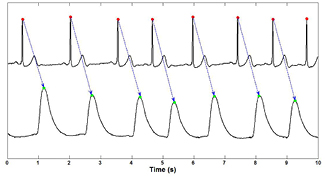
\includegraphics[scale=0.8]{images/sinkronisasi.jpg}
    \caption{Sinkronisasi antara ECG dan PPG}
    \label{fig:ecg_vs_ppg2}
\end{figure}

\section{Aritmia}
Aritmia adalah kategori gangguan jantung yang berupa tidak normal-nya irama jantung. Beberapa panyakit jantung yang tergolong aritmia antara lain:
\begin{itemize}
	\item \textit{Tachycardia} (detak lebih cepat dari normal),
	\item \textit{Bradycardia} (detak lebih lambat dari normal),
	\item \textit{Premature Atrial Contraction} (PAC),
	\item \textit{Premature Vantricular Contraction} (PVC),
	\item \textit{Ventricular Tachycardia} (VT) (detak ventrikel sangat cepat), dan
	\item \textit{Ventricular Fibrillation} (VF) (detak ventrikel tidak beraturan).
\end{itemize}

\textit{Premature Contraction} berarti siklus detak yang \textit{premature} (tidak pada waktunya) disebabkan oleh kontraksi pada atrium (bilik) atau ventrikel (serambi) terjadi lebih cepat atau lebih lambat dari seharusnya. \textit{Premature Contraction} tergolong serangan kecil (tidak berbahaya)[xx], sedangkan VT dan VF tergolong serangan besar (berbahaya). \textit{Premature contraction} yang terjadi berulang kali dan cepat merupakan awal dari peristiwa VT maupun VF. Contoh kemunculan PAC, PVC dan VF dapat dilihat pada gambar \ref{fig:contoh_aritmia}.

\begin{figure}[H]
    \centering
    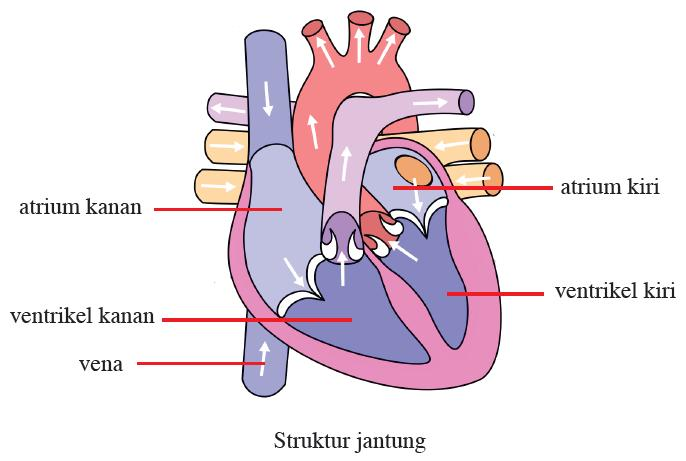
\includegraphics[scale=0.4]{images/jantung.jpg}
    \caption{Struktur jantung sederhana}
	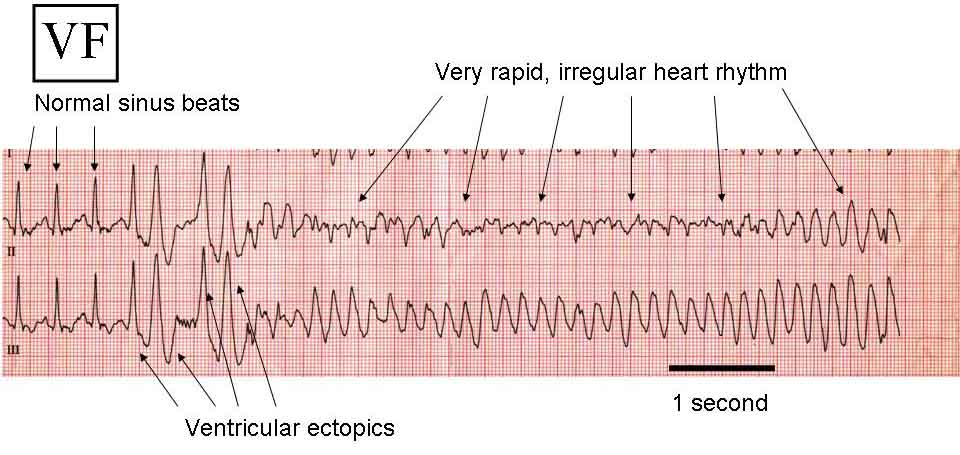
\includegraphics[scale=1.2]{images/VF.jpg}
    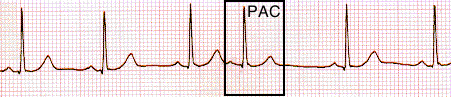
\includegraphics[scale=0.5]{images/PAC1.png}
	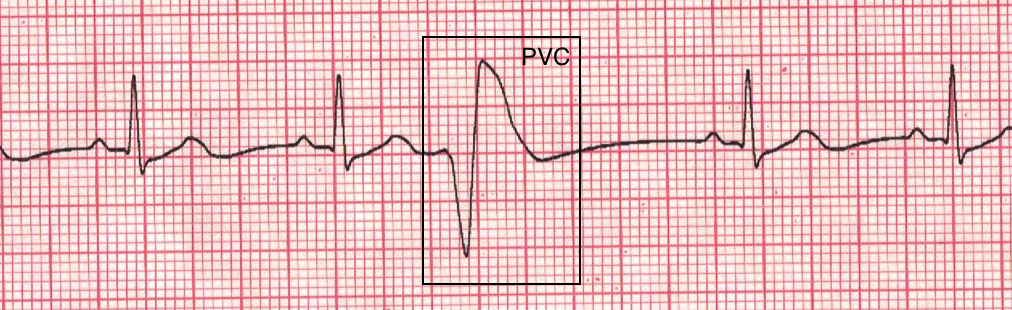
\includegraphics[scale=0.25]{images/PVC1.png}
    \caption{a. Sinyal VF; b. Sinyal PAC; c. Sinyal PVC}
    \label{fig:contoh_aritmia}	
\end{figure}


\section{Node.Js dan Mongo.Db}
Sebuah sistem monitoring yang dapat berjalan secara Ubiquitous haruslah dibangun dengan konsep \textit{Internet of Things} (IoT). IoT ialah konsep dimana objek objek (Things) dapat saling berinteraksi pada jaringan Internet tanpa membutuhkan manusia. Pada konsep IoT diperlukan setidaknya 3 komponen yaitu Sensor, Server dan Actuator. Sensor berfungsi sebagai pengambil data. Server yang menjalankan \textit{web service} (layanan web, contoh: http server, mqtt broker dan db server) berfungsi sebagai pengolah data. Actuator berfungsi sebagai pelaksana perintah dari server, seperti mengeluarkan suara dan membelokkan/memutus arus listrik. Node.Js dan Mongo.Db, keduanya dibutuhkan untuk membangun sebuah web service pada server.

\subsection{Node.Js}
Node.Js adalah teknologi Javascript (Js) \textit{Runtime} yang dibangun diatas Chrome V8 JS Engine. Node.Js memungkinkan bahasa pemrograman Js menjalankan web service. Node.Js dirancang menggunakan skema \textit{event-driven} dan \textit{non-blocking IO}, sangat sesuai untuk aplikasi \textit{data-intensive real-time} \cite{nodejs}. Node.JS juga telah terbukti secara performansi lebih cepat dari bahasa scripting lain seperti PHP, Python, dan Ruby bahkan tidak jauh lambat dibanding bahasa ter-\textit{compile} seperti JAVA, C, dan C++ \cite{node_comparisson}.

\subsection{MongoDB}
MongoDB adalah salah satu jenis program penyimpanan data yang bersifat NoSQL. MongoDB menyimpan data dengan bentuk dokumen dan format JSON. MongoDB dirancang untuk kasus penggunaan yang \cite{why_mongo}:
\begin{enumerate}
	\item Membutuhkan beban penulisan data yang tinggi,
	\item Skema data yang tidak stabil,
	\item Ukuran data akan menjadi sangat besar,
	\item Tidak memiliki seorang \textit{administrator}
\end{enumerate}

\begin{figure}[H]
    \centering
	
\includegraphics[scale=0.15]{images/nodejs.png}
    
\includegraphics[scale=0.3]{images/mongodb.png}
    \caption{a. Node JS; b. Mongo DB;}
\end{figure}

\section{ESP-12}
ESP-12 adalah salah satu tipe \textit{System on Module} (SoC) yang diproduksi oleh Espressif dari China. SoC berarti papan sirkuit yang telah terintegrasi oleh sistem tertentu. Kelebihan utama ESP ialah ukurannya yang kecil (16x24x3 mm) tapi dapat berfungsi sebagai \textit{controller} dan telah dilengkapi modul Wi-Fi. Hal ini memungkinkan komunikasi sensor-server melalui jaringan WiFi tanpa perlu menambah modul jaringan lagi.

\begin{figure}[H]
	\centering
	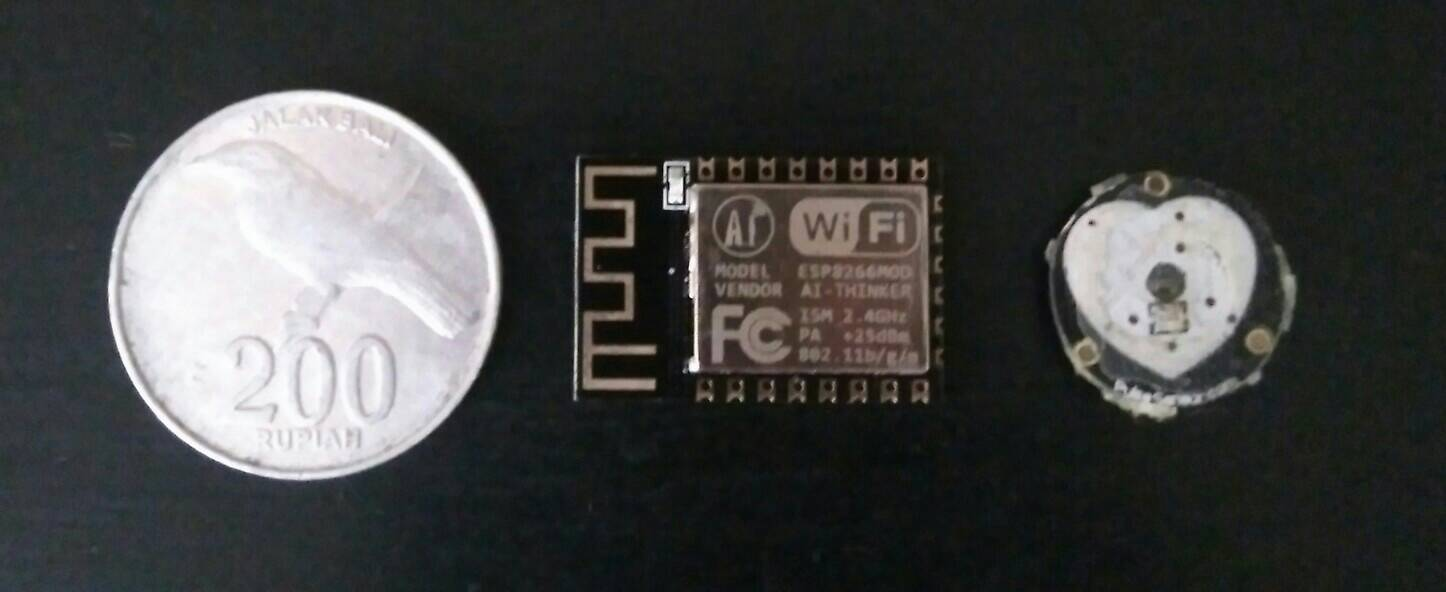
\includegraphics[scale=0.22]{images/coin_esp_pulse.jpg}
	\caption{Koin Rp200 - ESP-12E - Pulse Sensor}
	\label{fig:coin_esp_pulse}
\end{figure}

\section{Protokol MQTT}
Message Queuing Telemetry Transport (MQTT) adalah protokol transport
dengan skema komunikasi publish dan subscribe. MQTT dirancang menjadi protokol yang ringan, terbuka dan sederhana. Karakteristik ini membuat MQTT sangat tepat untuk digunakan sebagai protokol komunikasi machine-to-machine (M2M) dan Internet of Things (IoT). Protokol ini menggunakan TCP/IP pada layer transport. Terdapat tiga level Qualities of Service (QoS) dalam penyampaian pesan yaitu:
\begin{enumerate}
	\item QOS 0 atau “At most once”, dimana pesan dikirim dengan skema \textit{fire-and-forget} yang berarti tidak ada upaya menjamin pesan yang dikirim dapat sampai ke tujuan.
	\item QOS 1 atau “At least once”, dimana pesan dikirim dengan jaminan setidaknya pesan sampai sekali ke tujuan. Sehingga memungkinkan terjadinya duplikasi pesan di tujuan akibat pesan yang dikirim ulang dari pengirim.
	\item QOS 2 atau "Exactly once", dimana pesan dikirm dengan jaminan diterima tepat sekali ke tujuan. Sehingga tidak ada pesan yang terduplikasi di tujuan.	
\end{enumerate}

\begin{figure}[H]
	\centering
	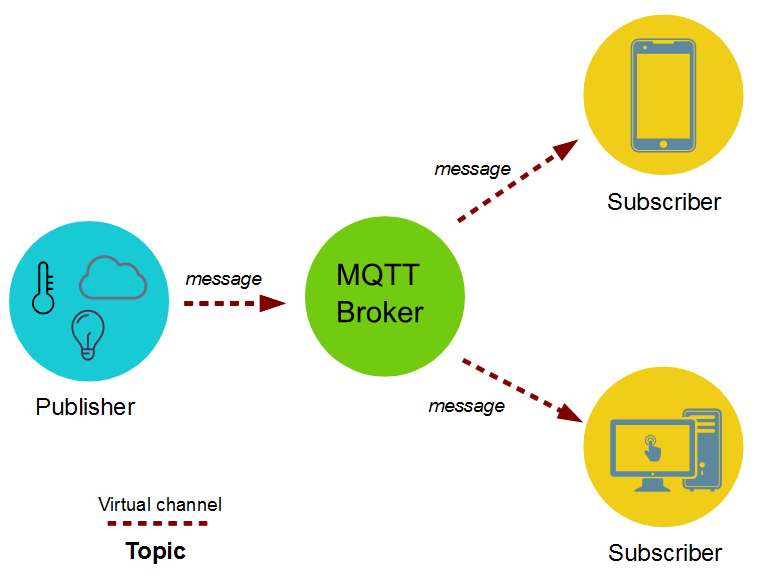
\includegraphics[scale=0.45]{images/mqtt.png}
	\caption{Cara kerja MQTT}
\end{figure}

